\section{问题三求解与分析}
\subsection{问题的描述与分析}

问题三保持场景 B 的 Task 与跨核同步结构，在 COPY\_IN 读共享输入时增加只读 L2 查询。Cache 命中走与 DDR 分离的读带宽池，未命中仍占用共享 DDR。FIFO 淘汰与容量决定后续复用能否发生；Cache 的时延收益不是命中次数的简单线性函数，因为并行 COPY 之间还会争用各自带宽。图~\ref{fig:q3-overview} 将共享读、FIFO 状态和同方案反事实比较连接到最终 Makespan。

% Generated figure only; description and reference belong before this input.
\begin{figure}[!htbp]
\centering
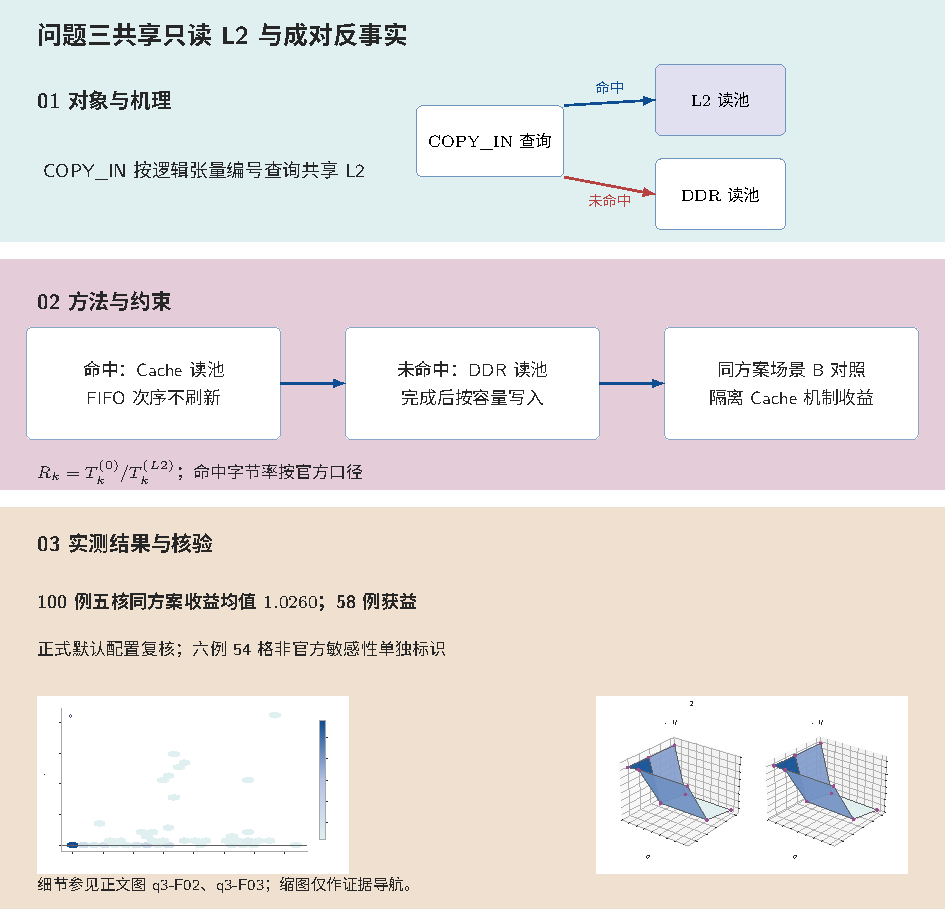
\includegraphics[width=160mm]{../求解/综合图/q3-overview.pdf}
\caption{问题三求解与核验总览}\label{fig:q3-overview}
\end{figure}
\FloatBarrier


存储层级的经典评价工作通过访问轨迹比较容量与替换策略下的命中行为\cite{mattson1970}。这启发本文同时报告L2命中字节和完成周期；然而题目使用不刷新次序的FIFO及两条独立读带宽池，不能直接把通用命中率公式套作本题的时延模型。

\subsection{只读 Cache 与成对评价模型}

对一次 COPY\_IN，先按张量逻辑编号查找 L2。命中时把所需字节交由 Cache 读带宽池，且不刷新该项 FIFO 顺序；未命中时从 DDR 读取，完成后按容量规则写入，只读 L2 不服务 COPY\_OUT。容量 $C_{\mathrm{L2}}$ 与读带宽 $B_{\mathrm{L2}}$ 由题定固定配置提供；单张量若大于容量就不缓存。DDR 的读写仍共享原带宽池，两个带宽池互相独立。

令同一图、同一核数和同一方案下，无 L2 与有 L2 的全局 Makespan 分别为 $T_k^{(0)}$ 与 $T_k^{(L2)}$。问题要求的 Cache 加速比是
\begin{equation}\label{eq:q3-cache-gain}
R_k=\frac{T_k^{(0)}}{T_k^{(L2)}}.
\end{equation}
另按官方口径，命中字节率为
\begin{equation}\label{eq:q3-hit-rate}
H_k=\frac{\text{L2命中 COPY\_IN 的字节数}}{\text{可查询 L2 的 COPY\_IN 总字节数}}.
\end{equation}
分母为零时按评估器的定义记录，不自行补造命中率。Cache 改变 COPY 完成顺序和全局争用，故 $R_k$ 未必与 $H_k$ 单调对应；结论依实际场景输出判断。

\subsection{方案适配与参数响应实验}

在固定官方配置下，对前两问的三个候选族重新用问题三评估器排序。选中方案之后，用完全相同的图和方案调用无 L2 的场景 B 评估器，再计算式~\eqref{eq:q3-cache-gain}，这样候选策略变化不会混入 Cache 收益。问题一、二、三各自可以选不同候选；若最终选中相同方案，仅说明该图上实测排序一致，不能推导一般情形必然相同。

容量与带宽的影响另做非官方参数敏感性实验：从正式 5 核案例按固定排序规则抽取不同 Cache 收益层的代表图，在工作区复制原配置后只改 L2 容量和读带宽。逐格对可用候选方案调用未改动的问题三评估器，记录固定默认方案的响应与该格重新择优的响应，并对比候选切换。它回答机制与方案适配方向；改动的配置不得并入题目要求的 100 例正式成绩，也不能用少量目的抽样推断 100 例平均收益。

\subsection{官方算例结果与分析}

在题定默认L2配置下，100例正式结果覆盖1至5核。五核平均加速比3.6104（无量纲），中位数$4.2231$，第10与第90百分位为$1.4609$、$5.0048$。其单核平均加速比为$1.0086$，可以高于1，因为分母仍是原始图的无L2单核基准。图~\ref{fig:q3-f06}按题目要求比较固定同一方案时无L2与有L2的1至5核平均加速比，两个序列都除以各算例原图无L2单核时间。图~\ref{fig:q3-f01}给出五种核数下同方案Cache收益比的经验累积分布；曲线在1附近快速上升，说明多数算例增益较小，而少数算例形成右尾。

\begin{figure}[htbp]\centering
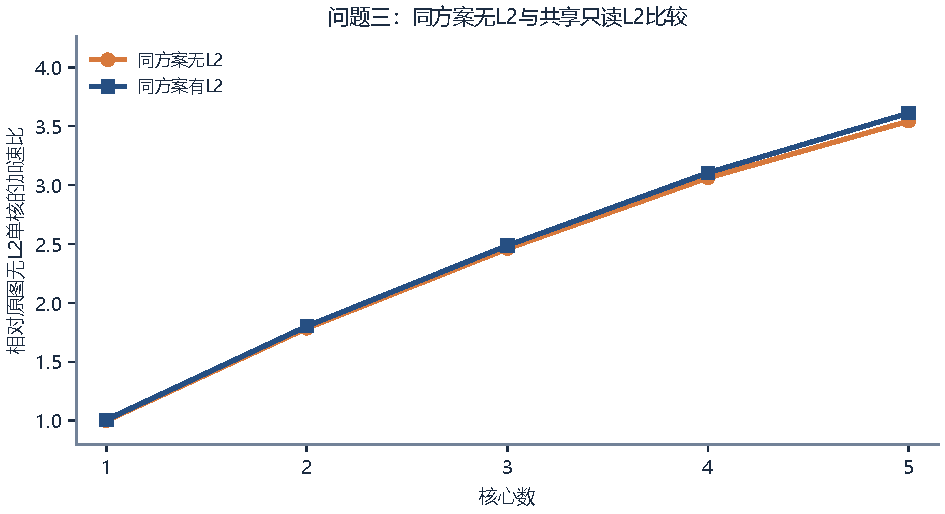
\includegraphics[width=160mm]{../求解/正式图件/q3-F06.pdf}
\caption{同方案无L2与有L2的核数比较}\label{fig:q3-f06}
\end{figure}

无L2与有L2曲线在核数1至5处的平均值分别为
\begin{align*}
(\bar S_k^{(0)})_{k=1}^{5}&=(1.0000,\ 1.7850,\ 2.4605,\ 3.0613,\ 3.5421),\\
(\bar S_k^{(L2)})_{k=1}^{5}&=(1.0086,\ 1.8026,\ 2.4873,\ 3.1044,\ 3.6104).
\end{align*}
两条线每个横坐标都使用相同算例与相同问题三选中方案；因此其垂直差异与方案重选无关。无L2曲线与问题二图~\ref{fig:q2-f06}接近但不完全重合，是因为问题二在无L2规则下选候选，而这里为隔离缓存机制固定问题三方案。这个细微差别也说明跨问题直接比较均值不足以识别单一硬件效应。

\begin{figure}[htbp]\centering
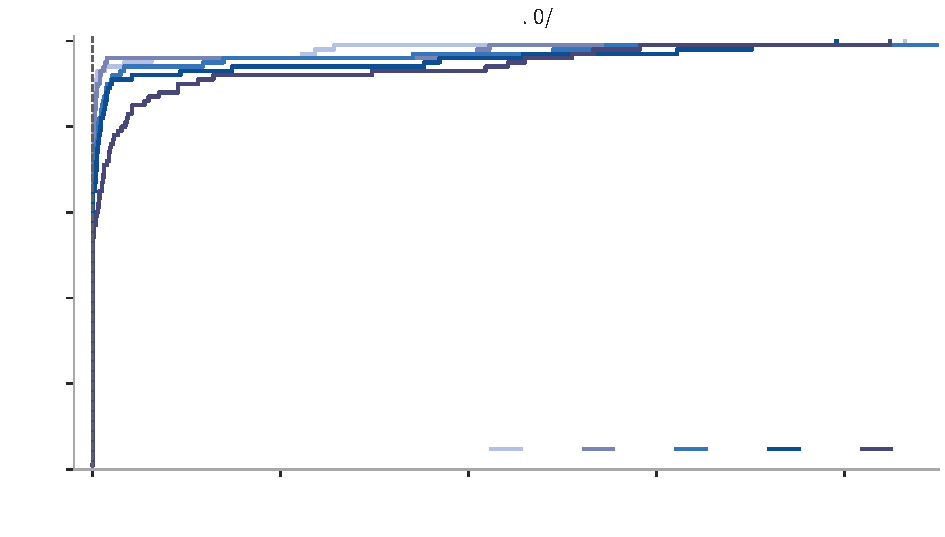
\includegraphics[width=160mm]{../求解/正式图件/q3-F01.pdf}
\caption{同方案Cache收益累积概率}\label{fig:q3-f01}
\end{figure}

五核同方案Cache比$R_5$均值为1.0260（无量纲），中位数$1.0001$，第90百分位$1.0464$；有正向收益的算例过半（58例）。平均逐例命中字节率为$21.29\%$，中位数$21.19\%$。最低$R_5$略小于1，表明FIFO与两个带宽池改变事件次序后，极小的逆向变化在官方模拟输出中确实可能发生。图~\ref{fig:q3-f02}把逐例命中字节率和同方案收益相对照。离散点与高密度区说明“命中率高”不是“完成时间按比例下降”的充分条件；还需看COPY是否落在关键路径，以及DDR/Cache带宽竞争与计算Pipe的重叠。

\begin{figure}[htbp]\centering
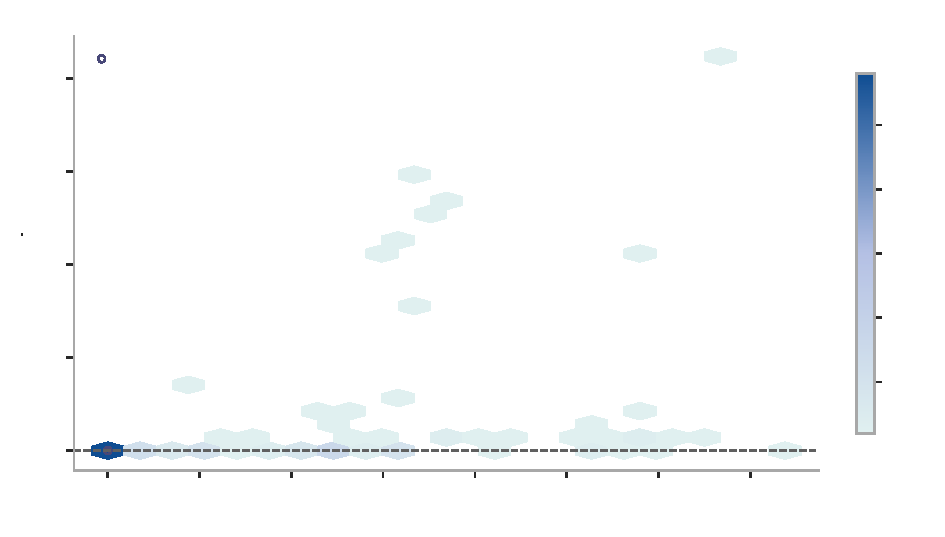
\includegraphics[width=160mm]{../求解/正式图件/q3-F02.pdf}
\caption{L2命中率与同方案收益}\label{fig:q3-f02}
\end{figure}

表~\ref{tab:q3-cache-cases}给出命中率与完成周期不能互相替代的逐例证据。算例083在固定的五核方案下，无L2与有L2分别需$442480$和$310731$周期，命中字节率$67.57\%$，收益比为$1.4240$。这证明在该案例的题定事件模型中，共享读开启后全局完工时间确实下降；汇总量本身还不能定位具体受益的关键事件。算例002也有$23.38\%$的命中字节命中，但总周期从$55096$微增到$55099$，收益比$0.99995$；三周期差异极小，不能据此声称缓存一般有害。两例共同支持只按命中比例排序的局限：被加速的读若不在控制全局完工的事件链上，其统计命中可以存在，而Makespan几乎不动。

\begin{table}[htbp]\centering
\caption{五核同方案L2收益的两端算例}\label{tab:q3-cache-cases}
\small
\begin{tabular}{c r r r r}
\toprule
算例 & 无L2周期 & 有L2周期 & 命中字节率 & 同方案$R_5$ \\
\midrule
083 & 442480 & 310731 & $67.57\%$ & 1.4240 \\
002 & 55096 & 55099 & $23.38\%$ & 0.99995 \\
\bottomrule
\end{tabular}
\end{table}

该成对比较在同一图、核数和方案上完成，故候选重选不是表中差异来源；但它也不是脱离评估器的物理芯片实验。FIFO淘汰次序、DDR与L2各自带宽以及并行COPY事件均由题定模拟规则决定，命中率只是其中一个过程变量。对高命中而低收益的图，应优先查看命中COPY是否位于关键依赖链，而不能自行把所有命中字节乘上一个统一的节省周期系数。

五核最终候选为连通块66例、深度分段26例、分批8例。图~\ref{fig:q3-f05}按核数分别累计命中与未命中的COPY\_IN查询字节；横条是100例求和后的字节量，右侧比例是总字节汇总率，不能同前段的逐例命中率平均数混读。五核与较少核心之间的差异兼有切图候选变化，不应全归因于缓存策略。

\begin{figure}[htbp]\centering
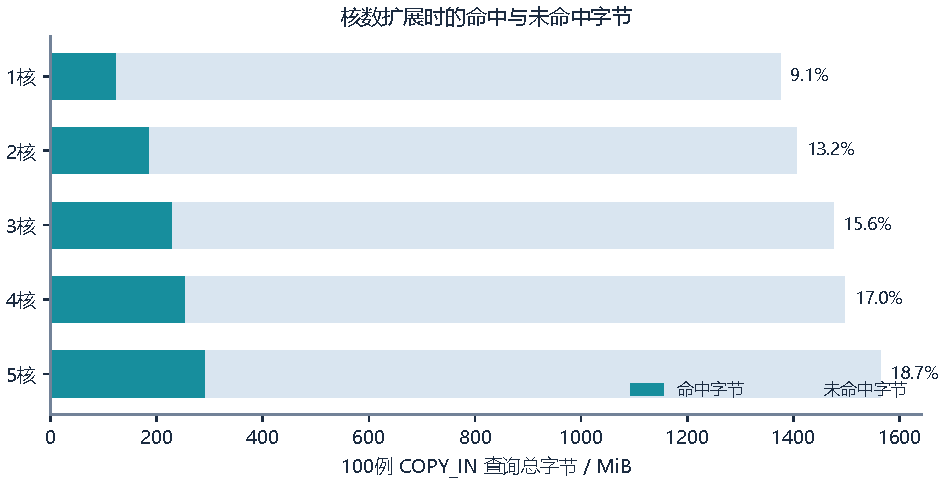
\includegraphics[width=160mm]{../求解/正式图件/q3-F05.pdf}
\caption{核数与L2查询字节}\label{fig:q3-f05}
\end{figure}

% Generated model comparison; edit scientific report and rerun the builder.
\noindent 本问是有显式约束和官方仿真目标的计算图组合优化；100 个图不提供最优方案标签，直接评价候选方案可复核，学习模型没有可验证的训练目标。\par


\subsection{逐核成对收益与命中含义}

Cache收益的正式统计必须把方案身份固定。对每个案例、核数先取问题三正式选中的$p$，分别在题定场景B无L2和有L2条件下评估$T^{(0)}(p)$、$T^{(L2)}(p)$，再形成逐例比值$R=T^{(0)}(p)/T^{(L2)}(p)$。表~\ref{tab:q3-core-deep}列出的均值是100个$R$的算术平均，而不是两个100例平均完成周期之比。两个汇总顺序不同：长图可能在平均周期中占主要权重，却在逐例比值平均中与短图各占一票。本文采用逐例求比的口径与原题加速比要求一致，因此不能用总命中字节数或总节约周期除以总时长代替。

\begin{table}[htbp]\centering
\caption{固定同一方案时的逐核L2收益分布}\label{tab:q3-core-deep}
\small\begin{tabular}{rrrrrr}\toprule
核数 & Cache比均值 & 中位数 & 受益/逆向例数 & 零命中例数 & 平均命中率 \\ \midrule
1 & 1.0086 & 1.0000 & 25/0 & 69 & 9.20\% \\
2 & 1.0120 & 1.0000 & 38/0 & 33 & 14.03\% \\
3 & 1.0143 & 1.0000 & 39/0 & 28 & 19.10\% \\
4 & 1.0190 & 1.0000 & 44/0 & 30 & 17.88\% \\
5 & 1.0260 & 1.0001 & 58/1 & 24 & 21.29\% \\
\bottomrule\end{tabular}\end{table}


从一核到五核，平均同方案收益依次为$1.0086$、$1.0120$、$1.0143$、$1.0190$、$1.0260$；严格受益案例数分别为25、38、39、44、58。这个趋势与图~\ref{fig:q3-f06}中两条平均加速比曲线的间距增大一致，但它们不是同一统计量：图~\ref{fig:q3-f06}分别对两种情景的$T_1/T_k$取均值，表中的收益则对同方案$T_k^{(0)}/T_k^{(L2)}$取均值。不同核数的方案本身会重新择优，因此从一核到五核的变化也不应被解释成“仅增加核心必然提高某张图的L2命中”。四核平均命中率$17.88\%$还低于三核的$19.10\%$，正说明不同分配、不同COPY访问序列会改变FIFO状态。

五核有24例命中字节率为零；在其余76例中，58例同方案时长改善，17例在记录精度下完全持平，1例出现极小的逆向差异。因而“有命中”既不是严格收益的充分条件，也不保证收益幅度与命中率成比例。计入命中率的字节可能属于非控制最后完工时刻的COPY，也可能与其它Pipe上的工作并行；从DDR转向Cache的读请求还会改变两个独立带宽池的排队与完成先后。算例002的$0.99995$是官方确定性事件模型中的三周期差异，不宜放大为稳定的硬件退化规律。反过来，算例083的$1.4240$也不能推广成“约68\%命中率通常带来42\%提速”，因为其它案例的依赖链与带宽竞争不同。

方案适配与缓存机制仍应分开评价。五核问题二与问题三的胜出候选族仅在1个案例不同，四核也仅在1个案例不同；这说明当前三种候选在默认L2配置下通常保留相同的胜出族，但“族名相同”不保证方案逐字节相同。因此本文在每一例的缓存收益分子、分母上固定问题三的实际方案，而没有假定问题二结果天然可作同方案对照。后续若扩大候选空间或改变Cache容量，候选切换次数都可能变化，必须重新进行这一成对评估。

\subsection{命中率分层的反例与统计边界}

图~\ref{fig:q3-f02}展示命中率与收益的联合形状；为核对离散点代表多少案例，表~\ref{tab:q3-hit-crosscheck}把正式五核的100例按命中字节率$H$分为四个互斥区间，并在每层重算同方案Cache比。分层阈值只是解释用途，不参与方案择优，也不是从网格敏感性实验中调出的参数。四层计数24、25、37、14之和恰为100。表中的“严格受益”按官方记录比值大于1计数，因而极小但真实的周期差异仍按其方向记录，不能把这一计数解释为统计显著性检验。

\begin{table}[htbp]\centering
\caption{五核命中字节率分层后的同方案收益}\label{tab:q3-hit-crosscheck}
\small\begin{tabular}{lrrrr}\toprule
命中字节率范围 & 例数 & Cache比均值 & 严格受益例数 & 最大Cache比 \\ \midrule
零命中 & 24 & 1.0000 & 0 & 1.0000 \\
$0<H\leq0.20$ & 25 & 1.0043 & 13 & 1.0642 \\
$0.20<H\leq0.50$ & 37 & 1.0459 & 31 & 1.2912 \\
$H>0.50$ & 14 & 1.0563 & 14 & 1.4240 \\
\bottomrule\end{tabular}\end{table}


零命中层的24例全部没有同方案时长收益，符合只读L2没有实际服务字节时的机制预期。低命中层$0<H\leq0.20$的25例中，仅13例严格受益，平均收益比$1.0043$；其余12例的COPY命中并未改变全局最后完成时刻。在$0.20<H\leq0.50$的37例中，31例受益，均值$1.0459$；高于$0.50$的14例全部受益，但均值也仅$1.0563$。各层平均值随命中率上升，是这100例的描述性关联；表内同层最大收益分别为$1.0642$、$1.2912$与$1.4240$，跨度显示命中率相近的图仍可能有很不同的时间收益。

具体而言，命中字节率的分子是成功由L2读出的总字节，不记录这些COPY位于哪条控制全局终点的依赖链，也不记录命中发生时DDR是否拥塞。用$H$预测时间至少还要知道命中读的事件位置、L2池占用、DDR池占用和与计算Pipe的重叠；本研究没有从汇总命中率逆推出这些不可观测的事件结构。高命中层14例全部改善不意味着“$H>0.50$是充分条件”，因为这个说法只在当前有限案例与给定配置下成立，换容量、带宽或FIFO访问次序就可能改变。表~\ref{tab:q3-hit-crosscheck}因此作为模型解释与反例核查，不能作为新的参数优化器。

\subsection{图结构与共享缓存收益的交叉核查}

问题一已经按最大弱连通块所占非COPY操作比例$f$划分四个结构组。为检验“容易切开的图是否一定更受益于共享L2”，本文沿用那四个预先使用的分界，而不根据缓存结果重新寻找最显著阈值；在每个组内只取官方五核的对应案例，分别计算逐例命中字节率和同方案收益比的算术平均。表~\ref{tab:q3-structure-cache}的四组人数为38、21、13、28，恰好覆盖正式100例，严格受益数加总为58，与不分组的原始统计一致。这种交叉核对也防止因结构分组遗漏案例而把小样本均值误作整体结论。

\begin{table}[htbp]\centering
\caption{五核图结构分组下的同方案Cache收益}\label{tab:q3-structure-cache}
\small
\begin{tabular}{c r r r r}
\toprule
最大连通块占比 & 案例数 & 平均命中字节率 & 平均收益比 & 严格受益数 \\
\midrule
$f\leq0.05$ & 38 & 24.48\% & 1.0279 & 20 \\
$0.05<f\leq0.20$ & 21 & 24.69\% & 1.0516 & 12 \\
$0.20<f\leq0.60$ & 13 & 22.71\% & 1.0244 & 9 \\
$f>0.60$ & 28 & 13.76\% & 1.0048 & 17 \\
\bottomrule
\end{tabular}
\end{table}


最大连通块占比大于$0.60$的28例，平均命中字节率为$13.76\%$、同方案收益比为$1.0048$；最分散的$f\leq0.05$组对应$24.48\%$和$1.0279$。在本组数据中，较分散的结构确实伴随较高的平均命中与收益，但它并不构成单调的性能定律：$0.05<f\leq0.20$组的平均收益$1.0516$高于最分散组的$1.0279$，两组平均命中率却十分接近。中间的$0.20<f\leq0.60$组也不能仅按$f$在两端之间插值推算；它只有13例，均值容易受个别图的访问路径影响。

组内正向案例数进一步揭示均值的限制。$f>0.60$组仍有17/28例严格受益，说明较大的连通块不等于共享输入完全没有重用；只是这些改善的总平均幅度较小。$f\leq0.05$组虽然平均收益较高，严格受益也只有20/38例，其中算例083的同方案比值达到$1.4240$，使组内分布出现明显右尾。若用一个结构阈值直接决定是否开启L2，既会错过高连通组中的实际受益图，也会把低连通但处于非关键读链的图误判为高收益。$f$刻画图能否按弱连通成分拆开，$H$刻画产生了多少命中字节，$R$才是完整事件时间线的结果；三者的层级不能互相替代。

上述关联还受到候选择优的条件化影响：各组在五核下使用的切图候选可能不同，改变跨核输入复用和COPY访问次序。表内每个$R$的分子分母仍固定同一问题三方案，所以缓存收益的成对定义未变，但跨组比较并未固定方案族，也未控制图规模、深度与原始COPY强度。它只能说明当前100例的结构异质性，不能把最大连通块占比解释为对Cache收益的独立因果作用。后续若要建立可迁移的收益预测器，需要在同一图上对多个候选与多个容量配置做成组评价，并保留关键读事件和FIFO状态轨迹；本文没有用现有汇总表冒充这些尚未完成的实验。

\subsection{参数敏感性与独立核验}

为考察参数响应，另取6例有代表性的正式五核图，在复制的配置上设置容量$256\,\mathrm{KiB}$、$1\,\mathrm{MiB}$、$4\,\mathrm{MiB}$与读带宽$60,250,500$字节每周期的九格组合。每格重新评估全部可用候选，共54条最优记录；默认$1\,\mathrm{MiB}/250$格同正式实验逐字节复核一致。所有参数变化均为非官方配置，没有混入题定100例成绩。

图~\ref{fig:q3-f03}给出案例044与083的实测三维响应面，图中高度刻度以千周期为单位。044在该网格的完成周期范围为$98948$至$132892$，083为$287606$至$442480$；响应并不平坦。三维表面只连接九个实际网格点，不能解释为连续空间中的已验证插值最优。图~\ref{fig:q3-f04}在固定读带宽250字节每周期时，对照六例容量变化下的命中字节率；它展示缓存状态的响应，不直接展示完成周期。再从九格结果读取时长：在默认容量下将带宽从250提高到500，044的完成时间比为$1.0402$，083为$1.0684$；在默认带宽下把容量从1MiB提高至4MiB，044没有可测改善，083改善约$0.91\%$。这说明命中率和完工时间属于不同层次的结果，参数响应不能由单一全局命中率预测。

\begin{figure}[htbp]\centering
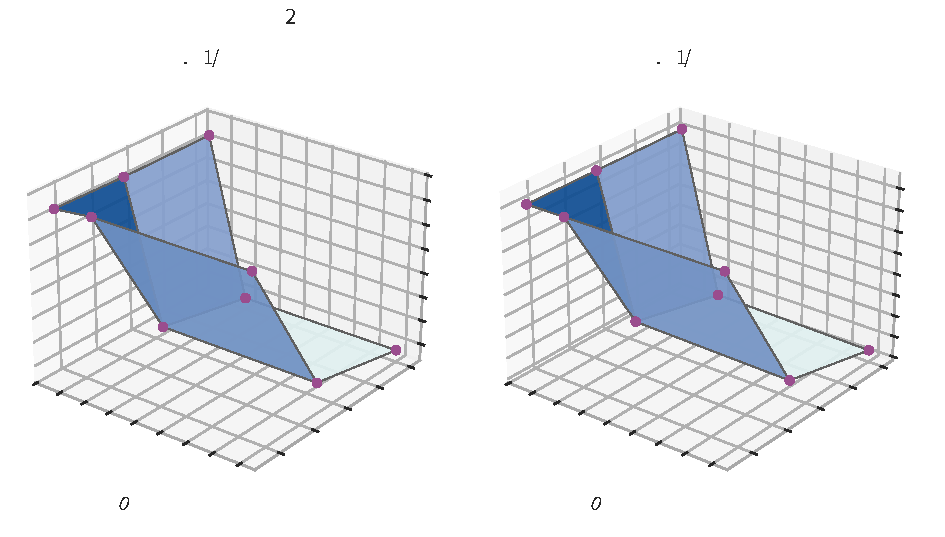
\includegraphics[width=160mm]{../求解/正式图件/q3-F03.pdf}
\caption{非官方L2参数响应面}\label{fig:q3-f03}
\end{figure}

\begin{figure}[htbp]\centering
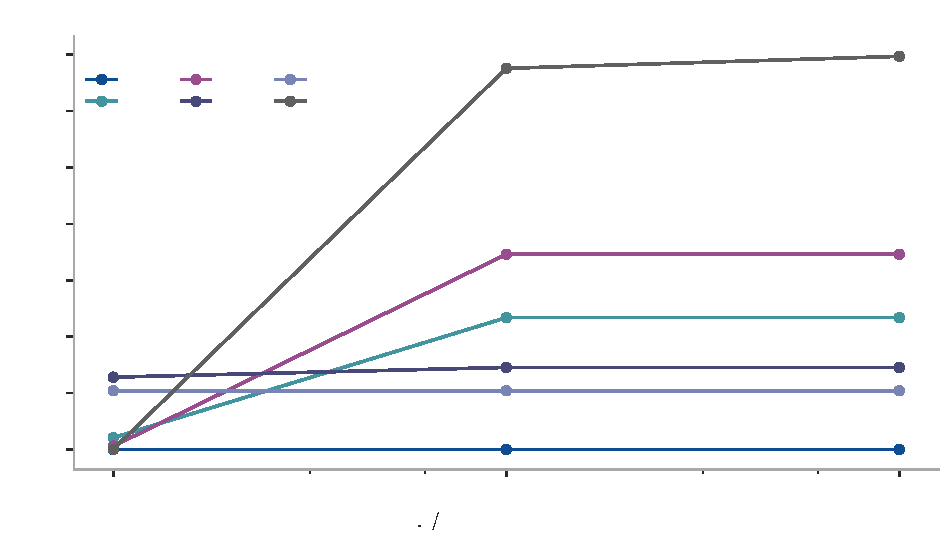
\includegraphics[width=160mm]{../求解/正式图件/q3-F04.pdf}
\caption{固定带宽下的容量与命中率响应}\label{fig:q3-f04}
\end{figure}

\subsection{有限网格内的条件差分}

为免把非官方网格误写成连续寻优，表~\ref{tab:q3-grid-deep}只在实际评价过的九个格点做有限差分。每一行的默认点是容量$1$ MiB、读带宽$250$字节每周期；“容量增益”指只把容量改到$4$ MiB时默认周期减少的百分比，“带宽增益”指只把读带宽改到$500$字节每周期时减少的百分比，均以本行默认周期为分母。表内还给出该案例九格完成时间的最小值和最大值，但区间端点未必来自同一参数轴，因此不可把“范围”当作某个单参数的因果效应。

\begin{table}[htbp]\centering
\caption{六例非官方L2网格在默认点附近的有限差分}\label{tab:q3-grid-deep}
\small\begin{tabular}{lrrrr}\toprule
算例 & 默认周期 & 九格范围/千周期 & 容量增益 & 带宽增益 \\ \midrule
001 & 47502 & 47.5--47.5 & 0.00\% & 0.00\% \\
002 & 55099 & 55.1--55.1 & 0.00\% & 0.00\% \\
044 & 102921 & 98.9--132.9 & 0.00\% & 3.86\% \\
050 & 84038 & 84.0--84.0 & 0.00\% & 0.00\% \\
056 & 219072 & 219.1--219.1 & 0.00\% & 0.00\% \\
083 & 310731 & 287.6--442.5 & 0.90\% & 6.40\% \\
\bottomrule\end{tabular}\end{table}


六例的响应强弱差别很大。算例001在九格中全部是$47502$周期，默认命中字节率为零；读带宽或容量在本次格点内改变，自然不会从这份记录产生可测收益。算例056虽有约$10.43\%$的默认命中率，九格也全部保持$219072$周期，说明其被L2服务的读在本评估范围内没有改变最后完成事件。算例002九格只跨$55099$至$55108$周期，算例050只跨$84036$至$84047$周期；相对于各自的总时长，这些变化极小。不能仅凭命中比例把这些案例排列成统一的性能响应顺序。

算例044和083构成另一端。044九格范围为$98948$至$132892$周期，在默认容量下提高带宽至$500$时完成时间降低$3.86\%$，而默认带宽下把容量增到$4$ MiB没有可测改善。083九格范围为$287606$至$442480$周期，带宽增益为$6.40\%$，容量增益为$0.90\%$；从默认带宽$250$反向降至$60$，在默认容量下其完成时间增加约$42.40\%$，044对应增加约$29.12\%$。这些数值揭示在当前两张图的固定方案和九格范围内，读带宽限制比容量增加更明显；然而其它四例并不呈现同样强的响应，故不对100例作平均参数结论。

该六例由正式结果的不同收益层选取，目的在覆盖机制表现，而不是对全体算例作随机抽样。每格既评估固定默认方案，也重新比较可用候选；在当前六例九格中，胜出候选族均没有切换，所以表~\ref{tab:q3-grid-deep}的时长变化主要对应参数路径而非候选族更换。仍需注意同族方案的具体排程在其它配置上可能改变，且格点之间没有额外试验，三维图面只供观察九点相邻关系。若将来增加容量或带宽范围、引入其它候选，必须重新检查默认格身份、候选切换以及官方与独立核验的一致性。把这一非官方实验与题定默认100例分开记录，是本文控制外推范围的必要条件。

独立程序逐格核对候选记录、配置副本和官方响应，54格统计审计通过；所选五百组方案的覆盖、时间线及官方响应交叉核验全部通过。共享L2只服务只读COPY\_IN，写回流量、私有缓存容量和无法共享的张量仍限制加速；本研究没有实测芯片功耗与物理时延，结论限定在题目给定的事件评估模型。




